%%%%%%%%%%%%%%%%%%%%%%%%%%%%%%%%%%%%%%%%%%%%%%%%%%%%%%%%%%%%%%%%%
% !TEX root = interimreport.tex
\clearpage
\chapter{THE LLVM COMPILER}\label{ch:Ch3}
%%%%%%%%%%%%%%%%%%%%%%%%%%%%%%%%%%%%%%%%%%%%%%%%%%%%%%%%%%%%%%%%%
%\vspace*{-12pt} % If no text above section, use this vspacing to lift the whole part to the proper starting point - SBÖ

LLVM is a collection of modular and flexible compiler and toolchain software that can be used to build a wide variety of compilers and other tools. LLVM compilers are organized into a set of libraries that implement the parts of a compiler. There are different front-end libraries a for every language and different back-end libraries for every architecture. There is only one common intermediate representation optimizer that connects specific front-end and back-end.

\begin{figure}
    \centering
    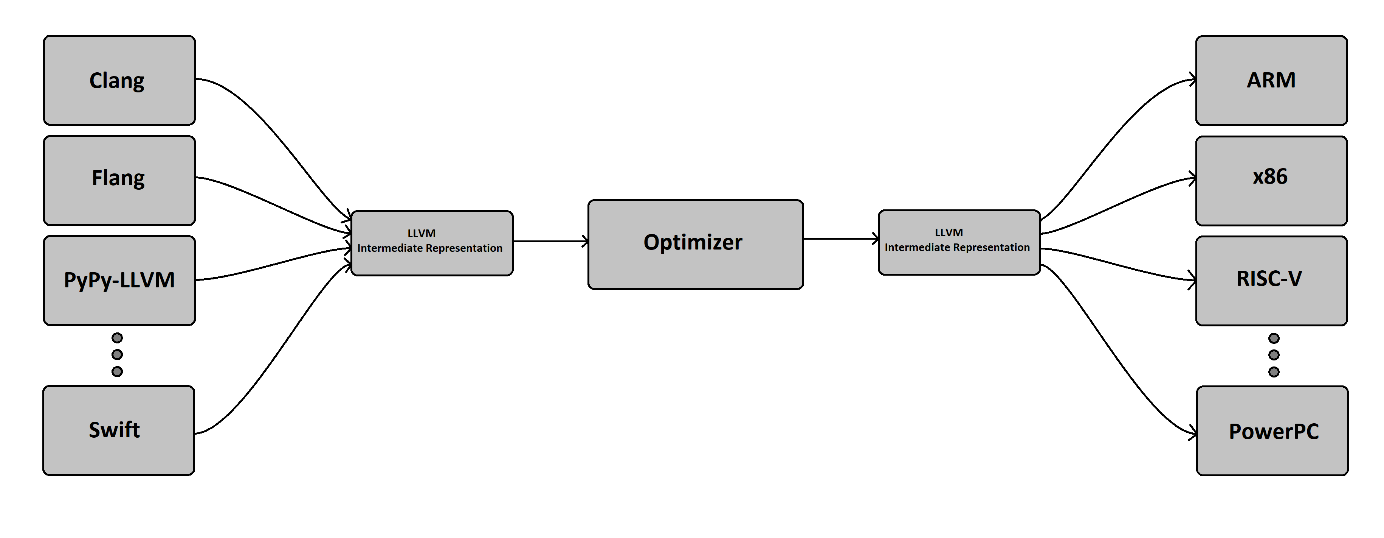
\includegraphics{the_llvm_compiler/llvm_diagram.png}
    \caption{Front-end and Back-end libraries connected by LLVM}
    \label{fig:llvm_diagram}
\end{figure}

LLVM IR is the common representation of languages. Various LLVM front-ends translate related languages into IR. Related back-end compiles IR into assembly according to the target hardware. This structure helps to increase flexibility between front-ends and back-ends. With this structure, we are able to have compilers for every combination of M source codes and N targets with M front-end and N back-end instead of M*N compilers. In our case, we do not have to struggle with the frontend also our backend will be working for every source code of LLVM because of this benefit. The front-end we use in the developing process will be clang which is the LLVM C/C++ front-end\cite{clang}.

\section{Parts of the Clang Frontend}

\subsection{Clang Lex Library}
Clang Lex Library is a typical lexer implemented as finite state machines that read source code one character at a time and transition between different states based on the characters read. The Clang lexer, which is a front-end compiler for the C, C++, and Objective-C programming languages, uses this approach to filter out comments and white space, recognize and tokenize language elements such as keywords, identifiers, and operators, and handle escape sequences and string literals. The implementation files of the Clang lexer can be found in the llvm-project/clang/lib/lex directory within the LLVM infrastructure.
	

\subsection{Clang Parse Library}

Clang Parse Library is the parser that takes the tokens produced by the lexer and constructs an abstract syntax tree (AST) to represent the structure and meaning of the source code. The Clang parser checks the source code for proper syntax and resolves symbols and identifiers. It also performs type-checking to ensure the source code follows the rules of the programming language. It creates the AST, a tree-like structure, that represents the source code in a way that is easily processed by the compiler. The implementation files of the Clang lexer can be found in the llvm-project/clang/lib/parse directory within the LLVM infrastructure.

\subsection{Clang Sema Library}

Clang Sema Library is a semantic analyzer that involves examining the meaning and context of the source code in a program. In Clang, semantic analysis is a phase in the compilation process that analyzes the abstract syntax tree (AST) generated by the parser to verify that the source code conforms to the rules of the programming language and is properly constructed. Semantic analysis performs various checks and transformations on the AST to ensure the source code is correct. The implementation files of the Clang semantic analyzer can be found in the llvm-project/clang/lib/sema directory within the LLVM infrastructure.

\subsection{Clang CodeGen Library}

Clang CodeGen is the code generation library that takes the abstract syntax tree which is generated by the parser and corrected by the semantic analyzer as input. It generates the intermediate representation code and produces .ll file which will be used in the backend. The implementation files of the Clang lexer can be found in the llvm-project/clang/lib/CodeGen directory within the LLVM infrastructure. 

\section{LLVM IR Optimizer}
LLVM Optimizer is a common optimization medium used for every possible source-target combination of a compiler. It takes the output file of CodeGen as input and runs three types of passes:

\begin{enumerate}
    \item Analysis passes: These passes analyze the IR and collect information about the IR without modifying the IR. 
    \item Transformation passes: These passes modify the IR by using the information gathered from Analysis passes. The optimizations are the product of these transformations. 
    \item Utility passes: These passes are used to perform tasks such as printing the IR or verifying the IR. 
\end{enumerate}

The output of the optimizer becomes the input for the target back-end which lowers the LLVM IR to the target Assembly. As the generated LLVM IR at the end of the optimizations is the object of pattern matching and assembly support for any custom instruction, it is a critical part of the design process.

\subsection{Analysis Passes}
There are almost 40 analysis passes. The significant documented analysis passes are listed below:

\begin{multicols}{2}
\begin{itemize}
\scriptsize
     \item Exhaustive Alias Analysis Precision Evaluator
     \item Basic Alias Analysis (stateless AA impl)
     \item Basic CallGraph Construction
     \item Count Alias Analysis Query Responses
     \item Dependence Analysis
     \item AA use debugger
     \item Dominance Frontier Construction
     \item Dominator Tree Construction
     \item Simple mod/ref analysis for globals
     \item Counts the various types of Instructions
     \item Interval Partition Construction
     \item Induction Variable Users
     \item Lazy Value Information Analysis
     \item LibCall Alias Analysis
     \item Statically lint-checks LLVM IR
     \item Natural Loop Information
     \item Memory Dependence Analysis
     \item Decodes module-level debug info
     \item Post-Dominance Frontier Construction
     \item Post-Dominator Tree Construction
     \item Alias Set Printer
     \item Find Used Types
     \item Detect single entry single exit regions
     \item Scalar Evolution Analysis
     \item ScalarEvolution-based Alias Analysis
     \item Stack Safety Analysis
     \item Target Data Layout

\end{itemize}
\end{multicols}

Some of the analysis passes will be discussed to provide background for the following sections.

\subsection{Transformation Passes}
There are almost 60 transformation passes. The documented transformation passes are listed below:

\begin{multicols}{2}
\begin{itemize}
\scriptsize
     \item Aggressive Dead Code Elimination
     \item Inliner for always\_inline functions
     \item Promote ‘by reference’ arguments to scalars
     \item Basic-Block Vectorization
     \item Profile Guided Basic Block Placement
     \item Break critical edges in CFG
     \item Optimize for code generation
     \item Merge Duplicate Global Constants
     \item Dead Code Elimination
     \item Dead Argument Elimination
     \item Dead Type Elimination
     \item Dead Instruction Elimination
     \item Dead Store Elimination
     \item Deduce function attributes
     \item Dead Global Elimination
     \item Global Variable Optimizer
     \item Global Value Numbering
     \item Canonicalize Induction Variables
     \item Function Integration/Inlining
     \item Combine redundant instructions
     \item Combine expression patterns
     \item Internalize Global Symbols
     \item Interprocedural Sparse Conditional Constant Propagation
     \item Jump Threading
     \item Loop-Closed SSA Form Pass
     \item Loop Invariant Code Motion
     \item Delete dead loops
     \item Extract loops into new functions
     \item Extract at most one loop into a new function
     \item Loop Strength Reduction
     \item Rotate Loops
     \item Canonicalize natural loops
     \item Unroll loops
     \item Unroll and Jam loops
     \item Unswitch loops
     \item Lower global destructors
     \item Lower atomic intrinsics to non-atomic form
     \item Lower invokes to calls, for unwindless code generators
     \item Lower SwitchInsts to branches
     \item Promote Memory to Register
     \item MemCpy Optimization
     \item Merge Functions
     \item Unify function exit nodes
     \item Partial Inliner
     \item Remove unused exception handling info
     \item Reassociate expressions
     \item Relative lookup table converter
     \item Demote all values to stack slots
     \item Scalar Replacement of Aggregates
     \item Sparse Conditional Constant Propagation
     \item Simplify the CFG
     \item Code sinking
     \item Strip all symbols from a module
     \item Strip debug info for unused symbols
     \item Strip Unused Function Prototypes
     \item Strip all llvm.dbg.declare intrinsics
     \item Strip all symbols, except dbg symbols, from a module
     \item Tail Call Elimination

\end{itemize}
\end{multicols}

\cite{passes}

\subsection{Case Study: Optimizations on S-box }\label{sbox-case}

\subsection{Clang Optimization Levels}

Clang can be invoked with optimization levels deciding which optimization passes are going to be run. The optimisations can target speed or code size. Speed optimising options range from "-O1" to "-O3". "-O2" enables most of the optimizations. "-O3" enables optimisations that can increase the compile time and generate larger code. Main code optimising options are "-Os" and "-Oz". "-Os" is similar to "-O2" but runs extra optimizations to reduce code size. "-Oz" runs more code reducing optimisations compared to "-Os" and is similar to "-O2" again \cite{clangCommands}.
Caution must be taken as when no arguments are given to Clang, at the time of writing, Clang uses the "-O0" optimization level. Implementing pattern matching on unoptimised LLVM IR is not feasible for several reasons. Firstly, the IR is more sensitive to changes in the frontend. Changing the code style in frontend can cause CodeGen to produce a slightly different IR which makes it less predictable. Secondly, the code size can be too large with redundant code which makes pattern matching large instructions cumbersome. We recommend using "-O2" or "-Os" optimization levels while developing instruction selection patterns. 




LLVM optimizer can be performed with opt [options] [filename] command\cite{optimizer}.

\section{Stages of the LLVM RISC-V Back-end}
LLVM RISC-V Backend is responsible for compiling optimized IR down to RISC-V assembly or object code. LLVM Backend consists of libraries for the code generation steps\cite{llvmbackend}.

\subsection{Instruction Selection}
SelectionDAG is the instruction selector of LLVM backends which is responsible for selecting the appropriate RISC-V instructions for a given intermediate representation instruction. It takes the target-independent LLVM code as input and generates the target-dependent DAG of instructions. SelectionDAG is the most important part of the compiler for us since we will be dealing with adding new instructions to the RISC-V Backend. 

\subsection{Instruction Selection}
SelectionDAG is the instruction selector of LLVM backends which is responsible for selecting the appropriate RISC-V instructions for a given intermediate representation instruction. It takes the target-independent LLVM code as input and generates the target-dependent DAG of instructions. SelectionDAG is the most important part of the compiler for us since we will be dealing with adding new instructions to the RISC-V Backend. 

\subsubsection{SelectionDAG construction}
After IR generating is done, SelectionDAG gets the optimized ir and converts it into target independent SelectionDAG representation. 

\subsubsection{SelectionDAG legalization}
SelectionDAG is a target dependent representation after the initial stage of the instruction selection. Before creating a target specific code, SelectionDAG checks if the DAG is legal because the constructed DAG may include incompatible instructions and data types to the target architecture. SelectionDAG legalizes the illegal DAG into a supported form. 

\subsubsection{SelectionDAG optimization}
SelectionDAG is in an optimizable form after legalization because legalization phase may create unnecessary DAG nodes and the reducable nodes are not combined yet. SelectionDAG optimizer minimzes the DAG nodes before creating the target spesific instructions.

\subsubsection{SelectionDAG target dependent instruction selection}
At the last phase of the instruction selection SelectionDAG selects the suitable instructions to the target architecture. SelectionDAG uses the relevant tablegen target description (.td) files to match the patterns and creates the target specific instructions.

\subsection{Scheduling and Formation}
Scheduling is the phase of assigning an order to the DAG form of RISC-V instructions. The formation phase is responsible for converting the DAG into a list of machine instructions.  

\subsection{SSA-based Machine Code Optimizations}
LLVM uses static single assignment (SSA) based optimizations before register allocation. SSA optimizations ensure that each variable is assigned and defined only once before it is used. 


\subsection{Register Allocation}
The register allocator of RISC-V back-end is responsible for assigning physical registers to virtual registers in the IR. Each target has specific register count and order. Register allocator maps the registers by taking the RISC-V architecture registers into account. It uses the relevant TargetRegisterInfo, and MachineOperand classes. Register allocation will play a key role in our project while we manipulating the implementation of the selected instructions.

\subsection{Prolog/Epilog Code Insertion}
Prolog and epilog code insertion is another optimization phase which is responsible for frame-pointer elimination and stack packing.


\subsection{Code Emission}
Code emission stage is responsible for lowering the code generator abstractions down to the MC layer abstractions. It takes the assembly as input and creates the final RISC-V machine codes. 

\subsection{Linking}
LLD is the LLVM linker library that is responsible for combining multiple object files into a single executable file. LLD is invoked after the code emission and generates a file by resolving symbol references, adjusting addresses, and performing other tasks as necessary.
